%%
\documentclass{aiaa-tc}% insert '[draft]' option to show overfull boxes
% \documentclass{article}% insert '[draft]' option to show overfull boxes
%%

% list packages between braces
\usepackage{graphicx}
\usepackage{varioref}%  smart page, figure, table, and equation referencing
\usepackage{wrapfig}%   wrap figures/tables in text (i.e., Di Vinci style)
\usepackage{threeparttable}% tables with footnotes
\usepackage{dcolumn}%   decimal-aligned tabular math columns
\newcolumntype{d}{D{.}{.}{-1}}
\usepackage{nomencl}%   nomenclature generation via makeindex
\makeglossary
\usepackage{subfigure}% subcaptions for subfigures
\usepackage{subfigmat}% matrices of similar subfigures, aka small mulitples
\usepackage{fancyvrb}%  extended verbatim environments
\fvset{fontsize=\footnotesize,xleftmargin=2em}
\usepackage{lettrine}%  dropped capital letter at beginning of paragraph
%\usepackage[dvips]{dropping}% alternative dropped capital package
%\usepackage[colorlinks]{hyperref}%  hyperlinks [must be loaded after dropping]
\usepackage{amsmath}

%% Daoru added the following package
\usepackage{multirow}
%%

\begin{document}

\title{CSCI545 Robotics Final Project Report\\
	Robotic Motion Planning}

 \author
{		May Ang%
		\hspace{3pt},
		Thomas Collins%
		\hspace{3pt},
		Justin Garten%
		\hspace{3pt},
		and Michael Joyce%
		\\
		\normalsize\itshape
		University of Southern California, Los Angeles, CA, 90007, USA\\
}
\maketitle

\begin{abstract}
In a world gone mad, one project dared to impose its own brand of
brutal justice on a world many thought too far gone to save.
\end{abstract}

\section{Introduction}
\label{Introduction}

\subsection{Background}

Robots are no longer confined behind striped yellow lines
with flashing lights to keep soft humans away from the moving
parts. They are operate in busy hospital hallways, kitchens, and homes
with pets, children, and clutter in a constant state of motion. As
such, the ability to evaluate and interact with those dynamic environments is
increasingly essential.

There are a number of possible approaches to this, many of which are
strongly influenced by the risks of the environment, nature of the
task, and the type of information to which the robot has
access. If uncertain, should it simply stop and wait for instructions?
Should it push through, trusting others to get out of its way? An
industrial bot capable of ripping through a wall might have very
different issues than a robotic vacuum which will at most scuff a
floorboard.

\subsection{Problem Description}

Issues relating to navigation and motion run up and down the entire
robotic stack. We chose to focus on the high-level planning aspects of
the problem, particularly relating to issues involved in dynamic,
noisy environments. Our primary approach was to explore, extend, and
evaluate three broad categories of methods for navigating in a dynamic
environment.

\subsection{Robocode Environment}

As our aim was to focus in on the planning and navigation algorithms,
we chose an environment which allowed us to abstract and encapsulate many
surrounding issues. The Robocode environment is a system designed for
simulated robotic tank tournaments. It offers flexible sensor and
control models and a relatively easily customizable environment.

Pieces:
- sensor model
- motion models (regular/advanced?)
- environment (discretization?)
- Bot coding issues
  - Threading for processing

Hm, how much to leave here versus individual sections?


\subsection{Report Outline}
In the following three sections, we discuss our efforts to explore
this task using Potential Fields, Markov Decision Processes (MDPs) and
reinforcement learning, specifically Q-learning.

\section{Potential Fields}
\label{Potential Fields}
Discussion and plots...

\section{Markov Decision Processes}
\label{Markov Decision Processes}
\subsection{Introduction}
Markov Decision Processes (MDPs) enjoy widespread use today in the field of robotics. Roboticists have found MDPs to be particularly useful in the realm of motion planning. 
The primary reason for this is quite apparent: MDPs allow roboticists to generate optimal motion plans even in the face of noisy robot motion. Noisy motion is a fact of life for physical robots, so
the ability to plan optimally in face of that uncertainty is of incredible importance. \\ \\
The class lecture slides, the homework, the \emph{Probabilistic Robotics} textbook, and even the seminal \emph{Artificial Intelligence: A Modern Approach} textbook only considered MDPs in the context of static environments whose layouts were known \emph{a priori} to the
robot. This is obviously not a realistic assumption. Navigating robots must deal with situations in which the goal is moving, the obstacles in the environment are moving, or both. In real-world navigation
applications, the world continues to transform as the robot figures out the best thing to do next. We wanted to investigate, in this part of our project, how effective MDPs could be in these types of online situations. More specifically, we wanted to investigate how well we could use MDPs  to track a moving enemy robot in a simulated world. The effectiveness of MDPs in online contexts is obviously
closely tied to the efficiency and computational complexity of the method used to generate optimal policies in those MDPs. For this reason, we focused our observation and experimentation primarily on how well value iteration performed in online contexts and experimented with real-time extensions to value iteration that made it converge significantly faster than the full algorithm.
\subsection{Setup}
One of the first and most important things we had to do to set up this part of the project was to discretize the state-space. The Robocode battlefield, as mentioned above, is a $600 \times 600$, 2-D plane of continuous (x, y) coordinates. If we had made our state set equal to the set of (x, y) coordinates of the Robocode battlefield, our MDP state-space would have been infinite. Though MDPs can be applied to infinite state spaces, such MDPs would certainly not be suitable for the kind of online applications we had in mind. Thus, we decided to split the battlefield into equal-size grid squares, each of which became one state in our state-space. We chose a state space consisting of 400 $30 \times 30$ point squares. The choice of $30 \times 30$ grid squares was not arbitrary. Robocode robots are, in fact, very nearly this size. We devised a tiling function that associated any (x, y) coordinate with one of these 400 states. One other thing regarding the state space is worth mentioning. Usually, given an (x, y) plane with a moving robot, you need to include the orientation of the robot (with respect to some fixed frame) as part of each state. This is not the case in the Robocode world because Robocode robots are capable of turning immediately to any orientation at any time. In fact, we made heavy use of this capability in our action set. \\ \\
Next, we had to discretize the actions of the robot. Robocode robots are capable of performing a number of actions, the most important of which are as follows: move ahead some distance, move back some distance, turn gun some number of degrees, turn radar some number of degrees, and 
turn body some number of degrees. Each of these actions takes a floating point argument (for distance or degrees), so the action space is also infinite. We knew that we would not be able to handle an infinite action-space in an online MDP, so we discretized the  action-space of the robot
as well. Since we were focusing on issues of motion planning, we decided to only consider movement actions as part of our MDP. Other necessary actions, such as sweeping the radar and firing the gun, were coded as purely reactionary or periodic. The robot swept its radar every 8 or so turns, and it fired straight ahead whenever it saw an enemy with its radar. We discretized the motion action-space of the robot into 8 actions: goNorth, goSouth, goEast, goWest, goNorthwest, goNortheast, goSouthwest, goSoutheast. Each of these actions moves the robot ahead a static amount in the specified direction. We decided that going backward, though possible in Robocode, was an unnecessary complexity, because turning 180 degrees and going forward is the same thing as backing up. Though we could have added added different actions that took the robot ahead different amounts in each direction, we wanted to keep the action set as minimal as possible in order to use it in an online, real-time fashion.
\subsection{Implementation and Experimentation}
The implementation of the functionality for this part of the project proceeded in five main steps, each of which added additional complexity to the environment, the test robot, or both. 
\subsubsection{Part I - Framework}
The first step we performed was to generate an MDP utility class (MDPUtility.java) that we could use for all of our MDP Robocode robot variations.
This involved developing, among other things, a simple reward function:
\begin{verbatim}
-100 for transitions from any state to the same state (hitting a wall)
100 for transitioning into a goal state.
-1 for all other actions	
\end{verbatim}
Next, we developed two different transition functions, one for noisy motion and one for non-noisy motion. The transition function for non-noisy motion is straightforward: each action in the MDP bot's action set takes the bot to one of the states surrounding its current state. For example, goNorth takes the MDP bot one state up (in the grid) and goEast takes the MDP bot one state to the right. Obviously, exceptions had to be made for the states surrounding the outside of the battlefield because some actions had the effect of keeping the MDP bot in the same state. The noisy transition function is similar to the non-noisy one but with the added complexity that the MDP bot has a 20\% chance of slipping each
time it takes an action. More specifically, with a probability of 0.2, each action the MDP bot takes leads it the it to the state immediately to the right or left (from the bot's point of view as it is heading straight forward) of the intended state. This transition function was very tricky to build because of all the special exceptions that had to be made for the states surrounding the edge of the battlefield. For example, consider taking the action goNorthwest in the state at the bottom left corner of the battlefield. With no noise, this action has a 100\% chance of putting the MDP bot back in the same state. With noisy motions, there is now a 10\% chance that the MDP bot will head straight North into a valid state. All these possibilities had to be enumerated. Once we had finished these functions, we used them to code value iteration in Java. This gave us a basic framework we could use to begin exploring the use of MDPs in the Robocode world. In order to validate the above MDP framework, we performed the following steps:
\begin{itemize}
\item Picked a goal state on the Robocode battlefield arbitrarily.
\item Ran value iteration offline with non-noisy and noisy transitions and saved the policies produced by each run.
\item Created two simple policy-following robots (MDPTestBot.java and MDPTestBotNoisy.java in the provided code base), one for non-noisy motions and one for noisy motions.
\item Set a stationary enemy robot at the goal state.
\item Plugged the noisy policy into MDPTestBotNoisy.java and the non-noisy policy into MDPTestBot.java and verified that, from any random starting position, each of our MDP bots went directly to the goal state. 
\end{itemize}
We ran the above experiments a number of times with different goal states to verify our MDP framework. Below are the non-noisy and noisy optimal motion policies produced for leading our MDP bots to state 273. Each vector in these figures represents which action the robot is supposed to take in each state. States are numbered from 0 to 399, starting at the bottom left corner and proceeding row-wise up to the top right. You can see that, in each case (noisy and non-noisy), the policy produced leads the MDP bot to the proper goal state. The optimality of the policies is easier to see in the non-noisy one. Notice how the non-noisy policy has our robot making a direct line to the goal along the directions of our 8 motion actions.  
\begin{figure}[htbp]
   \centering
   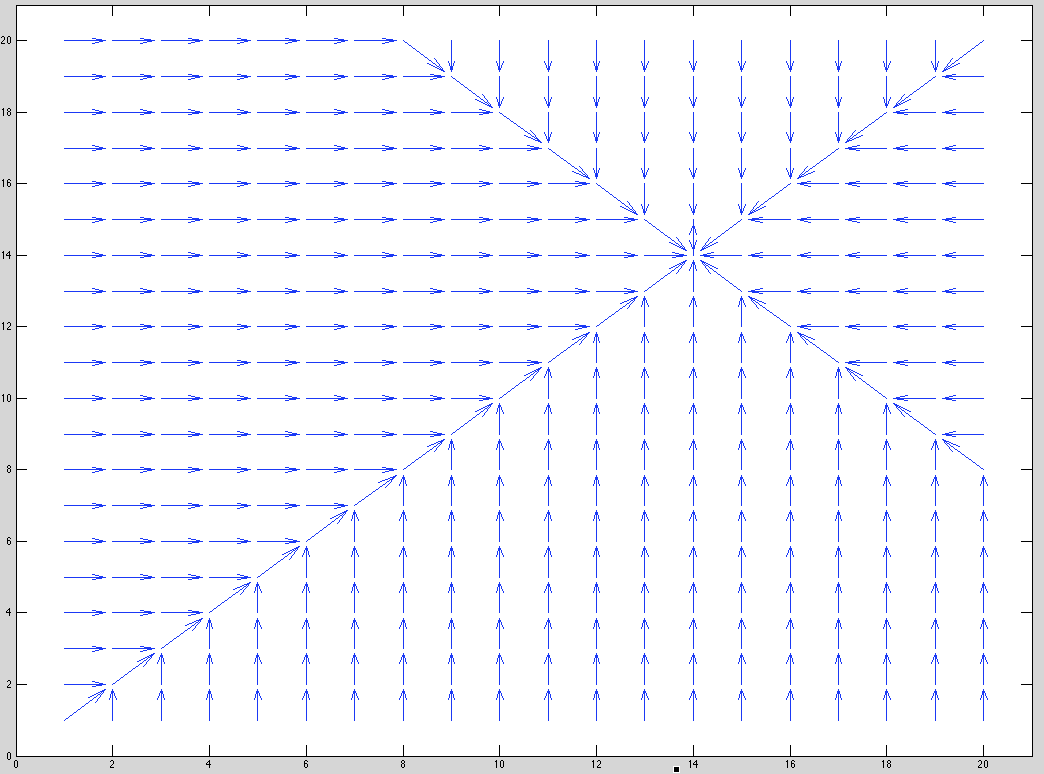
\includegraphics[width=170mm]{mdp_policy_to_state_273.png} 
   \caption{MDP Policy to lead an MDP bot to state 273. The motion of the MDP bot following this policy is assumed to have no noise.}
   \label{fig:sample}
\end{figure}
\begin{figure}[htbp]
   \centering
   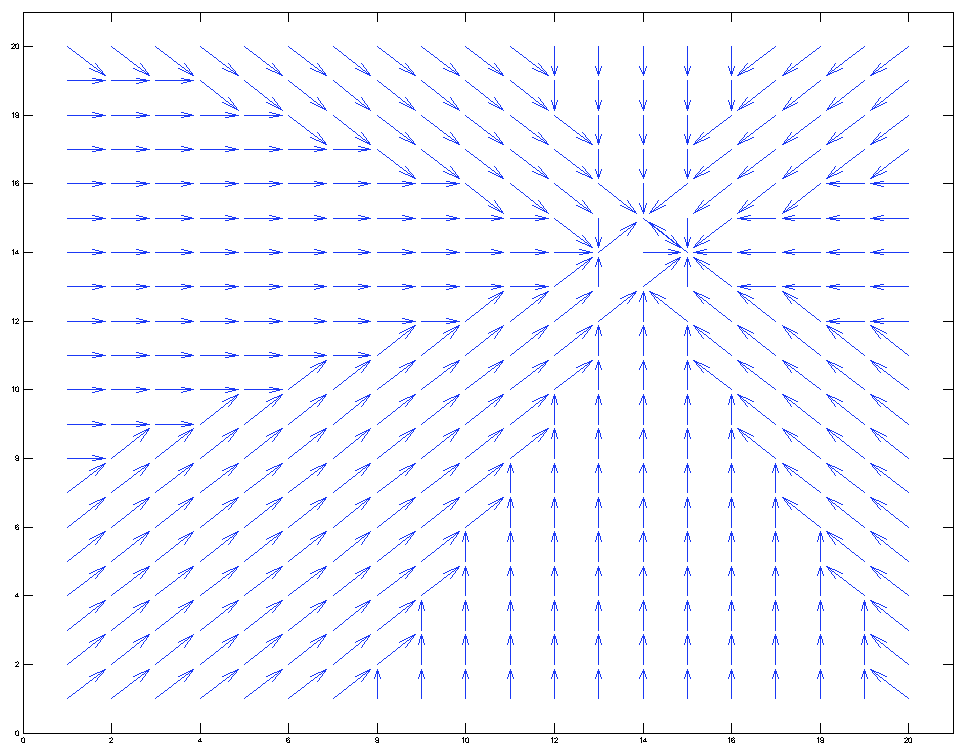
\includegraphics[width=170mm]{static_policy_noisy_to_state_273.png} 
   \caption{MDP Policy to lead an MDP bot to state 273. The motion of the MDP bot following this policy is assumed to follow the noise model described above.}
   \label{fig:sample}
\end{figure}
\clearpage
\subsubsection{Part II - Runloop Integrated Value Iteration}
The next main step we performed after developing and verifying our MDP framework was to find a way to run the value iteration "online" in the Robocode run loop. The first thing we tried was simply putting the value iteration function calls in the ScannedRobotEvent event callback function (triggered each time our MDP bot finds an enemy robot with its radar). This failed spectacularly because doing so blocked the main Robocode run loop of our bot. Our MDP bot was unable to take any actions during the time it was computing and was disqualified for skipping too many turns. We finally managed to integrate the full value iteration algorithm into a Robocode robot (MDPTestBotMovingTarget.java and MDPTestBotMovingTargetNoisy.java) by offloading the value iteration and policy calculations to a separate thread. We verified that we had successfully integrated value iteration into the Robocode run loop by doing the following experiment:
\begin{itemize}
\item Placed our MDP bot and the enemy bot in random locations on the map.
\item Had our MDP bot scan until it found the enemy bot.
\item Had our MDP bot calculate the (x, y) position of the enemy on the battlefield and find the corresponding state of the enemy robot.
\item Ran value iteration with the enemy's position state as our bot's goal state. This involved generating new rewards, a new Q-table, and a new policy.
\item Watched the MDP bot to make sure it went direcctly to the enemy position.
\end{itemize}
We performed the above experiment with non-noisy and noisy motion models, and we did it a number of times to make sure everything was working properly. This was a huge step toward our goal of running value iteration online with a dynamic environment.
\subsubsection{Part III - Moving Target Tracking}
The next step involved using value iteration online in order to follow a moving enemy bot. The implementation of this part was very similar to the implementation of the previous part, because we had already integrated value iteration into the Robocode run loop of a bot; however, there were a couple important changes we had to make to the code in order to make it follow a moving target. The most important change we made was to code in periodic radar sweeps. In general, generating a new policy through value iteration for a new goal state (new enemy position) took about 8 or 9 Robocode turns. So, every 8 turns we did a full 360 degree radar sweep of the battlefield to make sure that we had up-to-date information about the enemy's position. Before we added in the radar sweeps, our MDP bot was getting stuck forever at outdated goal states when the enemy took sharp turns. 
One interesting experiment we tried when developing this part of the code was predictive tracking. We tried running value iteration on the predicted goal state (based on the target's heading and velocity), rather than where the goal was when we started computing. We discovered that it was extremely difficult to estimate our own MDP bot's velocity because its motion is not smooth and because it continues following an outdated policy until the policy is updated. This made it almost impossible to estimate when we would reach the target position. We found that we got better performance with periodic radar sweeps and value iteration on the target's current position than with predictive targeting. The experiments we did for this part essentially consisted of running our MDP bot against a number of different basic enemy movements and verifying that our MDP bot followed the target without veering off in weird directions or getting completely stuck. We found no cases in which our robot was unable to follow the target effectively. We did this with both non-noisy and noisy motion models and had success with both. The code for this step can be found in MDPTestBotMovingTargetDynamic.java and MDPTestBotMovingTargetDynamicN.java).
\subsubsection{Part IV - Moving Target Tracking with Real-Time Optimizations}
The fourth step of this part of our project was where we experimented with "real-time" value iteration. As was mentioned above, the full value iteration algorithm took about 8 Robocode steps to converge. This is obviously not ideal because, in the time it takes to generate a new policy, the MDP bot has already taken 8 turns worth of non-optimized actions (not necessarily 8 distinct actions because, in Robocode, you can have a velocity of 8 points/turn at a maximum). We wanted to significantly cut down the time our MDP bots were following an outdated policy.  Thus, we implemented what we are calling real-time value iteration. Real-time value iteration essentially performs a local value iteration update on the following states: the previous enemy positon (old goal state), the new enemy position (new goal state), the states surrounding the old goal state, the states surrounding the new goal state, the states surrounding the states surrounding the old goal state, and the states surrounding the states surrounding the new goal state. The intuition behind this update is that, if we are close enough to the enemy robot, and the enemy robot has moved very little since we last saw him (i.e., the distance between the old goal state and the new goal state is very small), we need only update our MDP bot's policy in that area of the state space to optimally lead the bot to the new goal. As long as our MDP bot stays in that updated area, it will be following an optimal policy to the new goal state. More specifically, the real-time update works as follows:
\begin{itemize}
\item We update the reward values we have for the new enemy position (new goal state), old enemy position (old goal state) and two layers of states surrounding each of these states.
\item We run value iteration only over the states for which we updated reward values to update the Q-values for the states we are updating. The key to the effectiveness of this part is that we do the Bellman backup only over the states surrounding the state being observed, because we can only move to a state from the states surrounding it.
\item We use the updated Q-table to update the current policy to reflect new actions in the states we updated. 
This produces a policy that is locally optimized for the new goal state (in the area we updated) and optimized in all other parts for the old goal state. Here is an example of what an updated policy looks like graphically. The goal state was moved from state 190 (dead center in the quiver plot) to state 150 (two states down from state 190). In this figure, you can clearly see how the policy is optimized locally for state 150 (in a 5 by 9 rectangle around states 150 and 190), but globally for state 190. In particular, observe how the diagonal lines in the four corners of the plot are headed straight for the middle of the plot (state 190). This policy, for clarity purposes, is for a robot with non-noisy motion. However, the real-time update works equally well with noisy motion models.
 \begin{figure}[htbp]
   \centering
   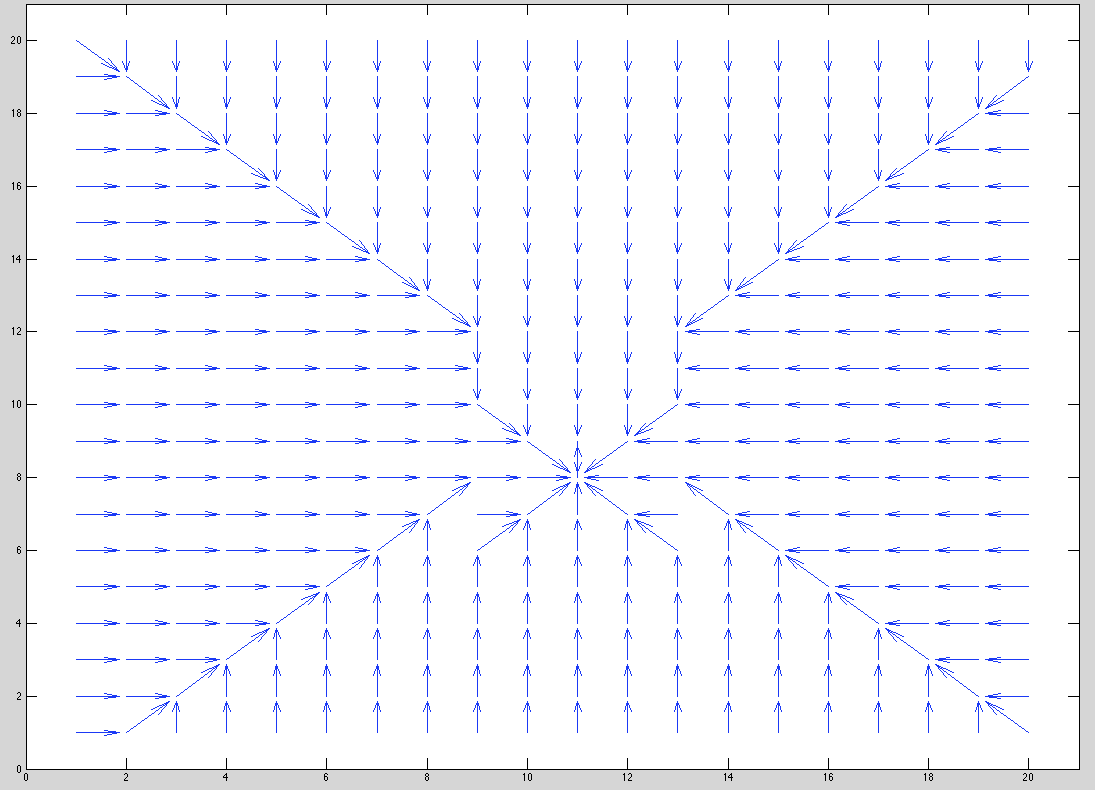
\includegraphics[width=170mm]{mdp_update_190_150.png} 
   \caption{MDP Policy that has been updated from goal state 190 to goal state 150 using our real-time value iteration function.}
   \label{fig:sample}
\end{figure}
\clearpage
\end{itemize}
We tested this procedure both offline and online. First, we tested it offline by running the full value iteration algorithm on a goal state, then running real-time value iteration to update that goal state. We saved both policies and verified that the latter policy was indeed a valid update of the former policy. 
Once we had tested this procedure thoroughly offline, we integrated it into new test bots (MDPTestBotRealTime.java and MDPTestBotRealTimeNoisy.java). Essentially, in these bots, we ran full value iteration to generate an initial policy and full value iteration every time the enemy was greater than 150 points away from our MDP bot. Once our MDP bot got within 150 points of the enemy, it transitioned to using the real-time value iteration update. The motion of our robot when it gets close to the enemy bot is noticeably more fluid in these bots because the real-time value iteration function converges in 0 Robocode turns. Our MDP bot is thus able to calculate an updated policy and start following that policy in the same turn. We ran this online, real-time experiment with a number of different enemy bot motions and with both noisy and non-noisy motion models. We saw some noticeable improvements to enemy tracking with the real-time value iteration algorithm when the enemy was moving straight away from our MDP bot (and was thus within our radar lock) and our MDP bot was close to the enemy bot. However, as was mentioned before, when the old goal state and the new goal state are too far from one another (perhaps because the enemy slipped out of our radar view for a few turns), the real-time update function fails, and the robot appears confused until it has time to do a full value iteration update. Consider the following figure. Here we have updated a policy from goal state 25 to goal state 31. Notice how all of the actions surrounding the old goal state have defaulted to going North. The new goal state is too far away from the old goal state to pull the actions around the old goal state in the direction of the new goal state. This is the major limitation of the real-time value iteration algorithm, and it is the reason we only used it in our MDP bots within a certain range. Based on our empirical evaluation of the real-time value iteration function, 5 states is as far of a jump as you can make (between old goal states and new goal states) without this improper behavior occurring around the old goal state. Again, for clarity, this figure is a policy for a noise-free motion model.  
 \begin{figure}[htbp]
   \centering
   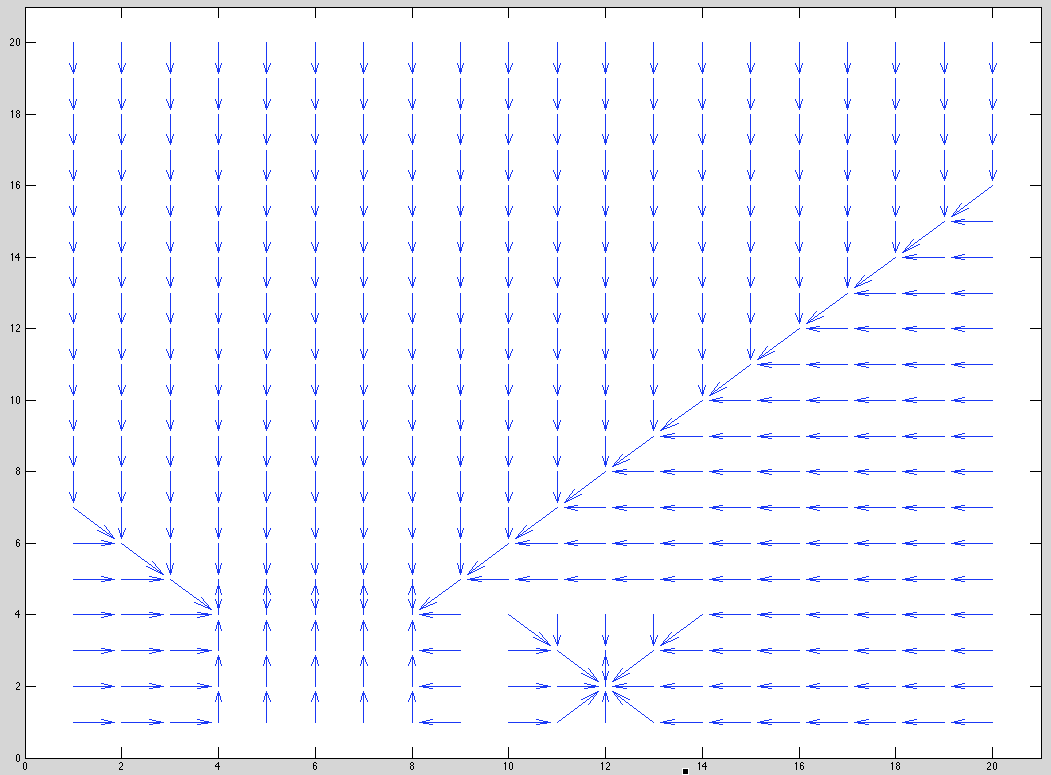
\includegraphics[width=170mm]{mdp_policy_update_25_to_31.png} 
   \caption{MDP Policy that has been updated from goal state 25 to goal state 31. With this large of a jump between goal states, the real-time value iteration algorithm fails.}
   \label{fig:sample}
\end{figure}
\clearpage
\subsubsection{Part V - Dynamic Obstacle Avoidance}
The fifth and final major step we took to implement MDPs in dynamic Robocode environments was to add in support for obstacle avoidance (moving or stationary obstacles). In the context of the Robocode environment, obstacles are simply other robots on the battlefield that we are not tracking. This was a major update to our current MDP bots because none of them had yet considered more than one other robot on the battlefield. We ended up representing these obstacles as a hash map. In Robocode, when a robot's radar discovers another robot, the name of that other robot is returned. Each of these names is guaranteed to be unique in the given battle. We used this name as the key of the obstacle and saved its current state as the value. We knew the name of the enemy we were tracking before the battle started, so we were able to distinguish this bot from all of the other bots. Every time we saw the same obstacle again, we updated its value (current state) in the hash map. This representation allowed us to track a list of obstacles (of arbitrary size) and their movement over time.  \\ \\
In addition to tracking objects and their positions over time, we had to factor them into our reward function. We wanted to ensure that this reward function made getting close to an obstacle bad enough that we avoided obstacles, but not so bad that we didn't risk going anywhere near them to track the target. We settled on the following updated reward function: 
\begin{verbatim}
-100 for transitions from any state to the same state (hitting a wall)
100 for transitioning into a goal state.
-20 for transitioning into an obstacle state
-20 for transitioning into a state surrounding an obstacle state
-20 for transitioning into a state surrounding a state surrounding an obstacle state
-1 for all other actions	
\end{verbatim}
These rewards make our MDP bots tend to avoid going within two states of obstacles on their way to the goal state. It is a very conservative reward function in the sense that it makes the MDP bot give itself a large buffer around obstacles. We also tested obstacle avoidance both offline and online. For our offline tests, we added obstacles to a hash map and ran value iteration with the new reward model to ensure that our policy was indeed pushing us away from the obstacles we specified and still leading us toward the goal. We tried this with different numbers of obstacles and obstacles in different locations. Once we were certain that was working, we integrated the obstacle avoidance reward structure and policy generation into new MDP bots (MDPTestBotDynamicOb.java and MDPTestBotDynamicObNoisy.java) and verified that obstacle avoidance worked in an online fashion. We tested our bots online with stationary obstacles and a stationary goal, stationary obstacles and a moving goal, a stationary goal and moving obstacles, and moving obstacles and a moving goal. In each test that we ran, it was readily apparent that our MDP bots were both avoiding the obstacles on the map and still heading toward the goal state. It is also worth mentioning one behavior that we noticed of these MDP bots. If the MDP bot tried to run value iteration when the goal robot was within one or two states of an obstacle, the MDP bot would just head straight North until it was able to see the enemy bot again a safe distance from any obstacle. We ran this test offline and verified that almost all of the actions defaulted to North in this case. This behavior makes sense. It is quite obvious that the MDP bot was unable to find a path to the goal that was not too painful reward-wise. It didn't know anything better to do, so it defaulted to going North in most states. Below you will find two figures. The first figure is a graphical representation of a policy that avoids two obstacles and leads to a goal. The second figure is a graphical representation of the policy produced when the goal-obstacle proximity problem described above is encountered. Both policies are for MDP bots with the noisy motion model described above.
 \begin{figure}[htbp]
   \centering
   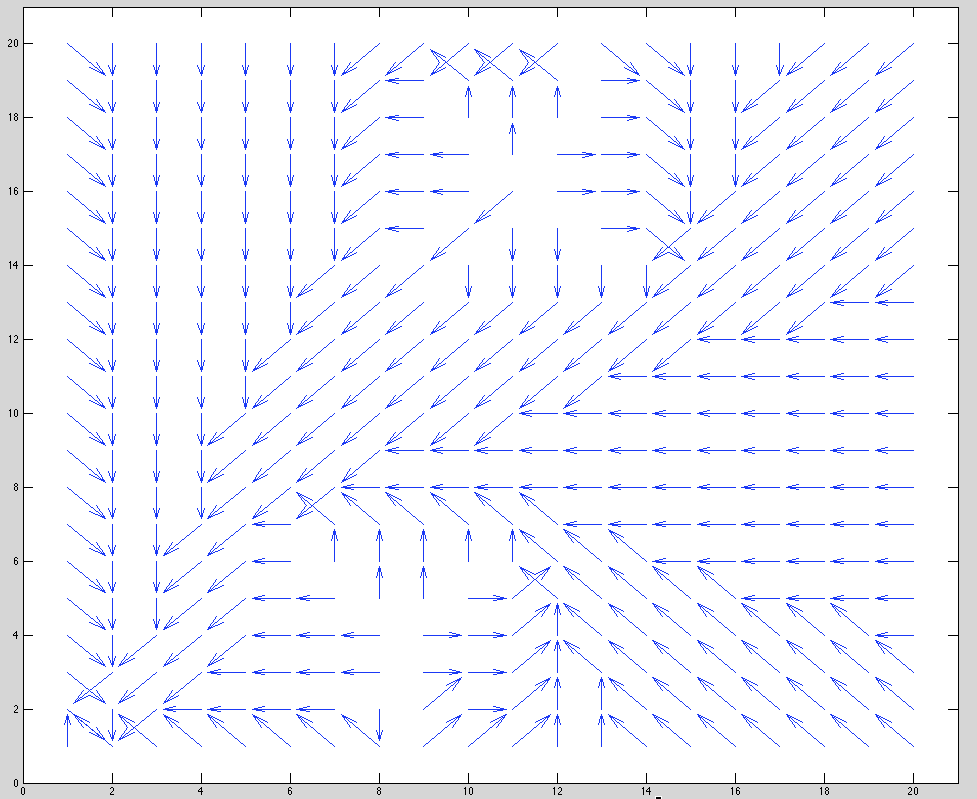
\includegraphics[width=170mm]{mpd_noisy_obstacles.png} 
   \caption{MDP Policy to lead an MDP bot to state 0 while avoiding obstacles at states 67 and 310.}
   \label{fig:sample}
\end{figure}
 \begin{figure}[htbp]
   \centering
   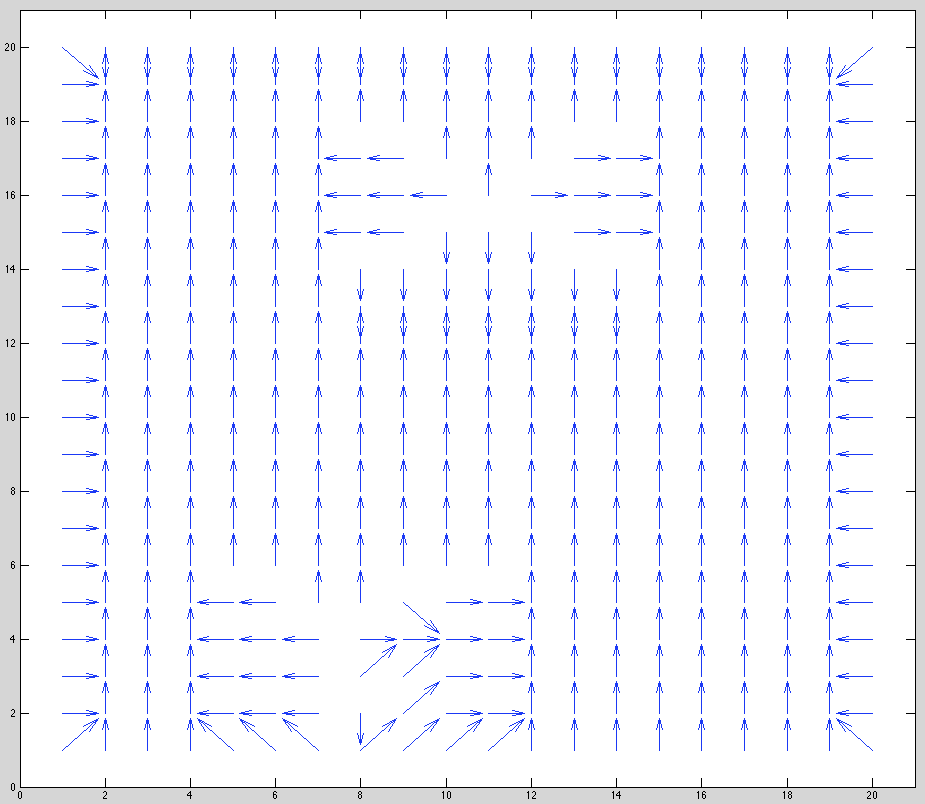
\includegraphics[width=170mm]{mdp_proximity_error.png} 
   \caption{MDP Policy to lead an MDP bot to state 68 while avoiding obstacles at states 67 and 310. The goal state is too close to the obstacles, and the path to the goal is obliterated.}
   \label{fig:sample}
\end{figure}

\clearpage
\begin{verbatim}

\end{verbatim}
As a final experiment, we attempted to code a real-time value iteration update that took obstacles into account. We took the real-time value iteration algorithm that we had built and modified it to also update the old and new states of the obstacles in the environment, as well as the states in the two rings surrounding the old and new states of each obstacle. Though we were able to get this function to converge in fewer iterations than the full value iteration algorithm, the results were non-intuitive. We speculate that perhaps the obstacles were too far away from the goal to update the obstacle locations in a way that was reasonable. There is also a possibility that the code itself is erroneous.
\subsection{Analysis}
In the Robocode environment, we were able to successfully implement a number of MDP bots that allowed us to examine the effectiveness of MDPs as a motion planning paradigm in different online motion planning and tracking contexts. In the preceding experiments, we discussed many of the things we learned about utilizing MDPs in an online way and many of the problems we encountered in doing so. In general, we found MDPs to be effective (in the sense that they successfully did what we wanted them to do) but relatively slow. This came as no real shock to us. Consider the computational complexity of the value iteration algorithm, particularly the inner loops. Let $s$ be the number of states and $a$ be the number of actions in the MDP. The computational complexity of these inner loops is $\Theta(s^2a)$. This clearly does not scale well as the number of states and actions increases. This computational complexity must also be multiplied by the number of times the outer while loop runs. For our MDP setup in the above experiments: 400 states, 8 actions, a 0.9 discount factor, and a Bellman residual of 0.01, it took 114 iterations of this outer while loop for value iteration to converge (116 iterations for the noisy motion model). Lower Bellman residual values caused this number of iterations to balloon. This is why the MDP bots we created were relatively slow to react to sudden changes in enemy position and obstacle position. The MDP bot had to consistently follow an outdated policy for several turns before it figured out how to get to the new goal. If the enemy took a sharp turn and moved at the maximum rate of 8 points per Robocode turn for 8 turns, it could be 64 points (about 2 states) away from the last place our MDP saw it before our bot figured out that it needed to turn and go a different direction. This accounts for the lack of fluidity in the MDP full value iteration tracking performance we saw and the relative ease with which our MDP bot lost track of the target when the target took sharp turns. On the other hand, full value iteration still worked surprisingly well. The full value iteration MDP bots we built do a decent job of following the target, even in the face of obstacles, provided that the MDP bot moves at least as fast as the enemy bot. Though 8 turns worth of suboptimal MDP bot action is clearly not ideal, it was not enough time for the enemy to get so far away that our MDP bot could never catch up again.  \\ \\
Still, we were unsatisfied with the performance of the full value iteration algorithm. One of the goals of our project was to make MDPs work in real-time. This meant that the MDP robot had to be able to update its policy \emph{and} follow that new policy in the same turn. In order to do this, we needed to find a way to boil down the aforementioned  value iteration algorithm to essentially a constant operation. The algorithm we developed, the specifics of which are discussed above, does a local policy update on 50 states: the new goal state, the old goal state, and the states in the two rings of states surrounding each of the old goal state and the new goal state. This algorithm creates a locally optimized policy for the new goal state and leaves the remainder of the policy optimized for the old goal state. If the old goal state and the new goal state are close together, this generates a global policy that can best be described as nearly or approximately optimized for the new goal state. Though this method is probably most useful in situations in which the MDP bot is very close to the enemy (which is how we made use of it), it could theoretically be used successfully at large distances. The beauty of this method is that it converged in 0 Robocode turns. It is therefore a full-fledged real-time value iteration procedure, at least for our (admittedly) small state-space and action-space. Notice that, though this is a constant operation with regards to state-space, increasing the size of the action space does affect the running time of this algorithm. As was mentioned above, this algorithm greatly increased the fidelity, reaction time, and smoothness of our MDP tracking when our MDP bot was close to the enemy and the enemy was within the radar scope of our MDP bot. With the completion of this method and the introduction of obstacles as a stress test, we had accomplished everything we set out to do in the MDP part of our project and gathered some great results.

\section{Q-learning}
\label{Q-learning}


\section{Conclusion}
\label{Conclusion}
To sum up...

\subsection{Future work}

\section{Acknowledgments}
Our team would thank Franz Kafka, Alan Turing, and the Ghost of 	
Christmas Past for their unwavering support during this project. We
would also like to pour a drink for our homies in the ground.


\end{document}